\documentclass[preprint,12pt]{elsarticle}
\journal{Future Generation Computer Networks}
\usepackage{amsmath, amsthm, amssymb,  graphicx}
\usepackage{subfigure}
%\usepackage{subfig}
%\usepackage{cite,citesort}
%\usepackage{cite}
\usepackage{multirow}
\usepackage{epsfig}
%\usepackage{epstopdf}
%\usepackage{algorithmic}

\usepackage{url}

% *** SPECIALIZED LIST PACKAGES ***
%
\usepackage{algorithmic, algorithm}
\begin{document}

\begin{frontmatter}

%% Title, authors and addresses

%% use the tnoteref command within \title for footnotes;
%% use the tnotetext command for the associated footnote;
%% use the fnref command within \author or \address for footnotes;
%% use the fntext command for the associated footnote;
%% use the corref command within \author for corresponding author footnotes;
%% use the cortext command for the associated footnote;
%% use the ead command for the email address,
%% and the form \ead[url] for the home page:
%%
%% \title{Title\tnoteref{label1}}
%% \tnotetext[label1]{}
%% \author{Name\corref{cor1}\fnref{label2}}
%% \ead{email address}
%% \ead[url]{home page}
%% \fntext[label2]{}
%% \cortext[cor1]{}
%% \address{Address\fnref{label3}}
%% \fntext[label3]{}

\title{Low-Carb: A Practical Technique Reducing Cellular Networks' Energy Consumption}

%% use optional labels to link authors explicitly to addresses:
%% \author[label1,label2]{<author name>}
%% \address[label1]{<address>}
%% \address[label2]{<address>}

\author[LUMS]{Muhammad Saqib Ilyas\corref{cor1}}
\cortext[cor1]{Corresponding author}
\author[LUMS]{Ghufran Baig}
\author[LUMS]{Zartash Afzal Uzmi}
\author[LUMS]{Ihsan Ayub Qazi}
\author[WaridTel]{Bilal Rassool}
\address[LUMS]{\ead{\{saqibm, 000000, zartash, ihsan.qazi\}@lums.edu.pk}School of Science and Engineering, LUMS, Lahore, Pakistan}
\address[WaridTel]{\ead{bilal.rassool@waridtel.com}Warid Telecom, Lahore, Pakistan}



\input{Sections/Abstract}
\begin{keyword}
%% keywords here, in the form: keyword \sep keyword

%% MSC codes here, in the form: \MSC code \sep code
%% or \MSC[2008] code \sep code (2000 is the default)
Green communication, BTS power-saving, energy conservation
\end{keyword}

\end{frontmatter}

%%
%% Start line numbering here if you want
%%
% \linenumbers

%% main text
\section{Introduction}
\label{sec:intro} 
Cellular networks are quite energy inefficient and consume several tens of TWhs of electrical energy
every year worldwide~\cite{Oh:Comm:2011}. This is a source of concern not only due to ecological concerns of global warming but also due to rising operational expenditure resulting from rising fuel and electricity prices. 

In the present work, we focus on the second generation (2G) cellular network technology, Global System for Mobile communication (GSM). While most recent research focuses on later generations of cellular networks, we focused on GSM for the several reasons. First, it has a large consumer base. Second, upgrade to later generations of cellular networks is prohibitively expensive especially for operators in the developing world where profits are low due to cut-throat competition and slow return on investment. Our proposed energy efficiency improvement framework is generic and should be applicable to other types of cellular networks as well, but we make no claim to its effectiveness in such scenarios. 

The major sink of power in a cellular network are Base
Transceiver Stations (BTSs), accounting for 50\% to 90\% of
the total power
consumption~\cite{Louhi:2007:BTSPower:INTELEC,Oh:Comm:2011}. Our focus in the present work is to reduce the energy consumption of BTSs to improve the overall cellular network's energy efficiency.

In a GSM network, every BTS is equipped with several transceivers (TRXs), each of
which is allocated a single frequency band for transmission and
reception of radio signals. Each TRX further uses time
multiplexing to handle up to 8 full-rate voice calls over its
assigned frequency band in GSM systems. A typical configuration
is ``6+6+6'' depicting a BTS serving three \textit{sectors}
each with six TRXs. Thus, a BTS offers a \textit{fixed} capacity, as
determined by the total number of TRXs installed. Sites are
deployed such that this fixed BTS capacity can handle the peak
traffic load. However, traffic peaks only for a short duration
dropping off to a much lower trough each day, which means that
the GSM networks are over-provisioned during
low-traffic regimes.

Over-provisioned BTSs would be fine if they also
consumed little power at no traffic
load. However, according to~\cite{Peng:2011:BTSSaving:Mobicom}
the no-load power consumption can be as high as 95\% of that at
full load. With fixed BTS capacity that is over-provisioned for
low traffic loads, today's cellular networks are highly energy inefficient.

There are generally two approaches to improve cellular network
energy efficiency. First is a clean-slate redesign which includes
innovations in communication systems, circuits and components.
This approach is not attractive for existing GSM operators,
which are the most prevalent in the developing world and are
expected to stay as such for several years to come, primarily due to the required expensive upgrades. 
A second approach is to make optimizations to the existing system
and equipment to get an improvement in overall energy
efficiency. Our present work is aligned with this latter
philosophy.

One can improve the energy efficiency of a cellular network by
adapting its ``online'' capacity to changes in traffic load.
Recent work has proposed turning off base stations to reduce
energy consumption during times of low traffic
load~\cite{Louhi:2007:BTSPower:INTELEC,Oh:Comm:2011,Peng:2011:BTSSaving:Mobicom,He:CellularPower:JN:2012}.
However, our conversations with multiple network operators
indicate that they are reluctant to employ such techniques
citing three reasons:
\begin{itemize}
\item Power cycling of entire base stations is expected to
    reduce equipment life time.
\item Turning off some BTSs may require an increased uplink
    power which may not be handled by many low-cost/power-limited mobile
    stations (MSs). This raises a risk of customer churn and is
    not acceptable to the operators in cut-throat
    competition prevalent in today's market.
\item These techniques of turning off BTSs may
    underestimate the increase in power needed for indoor
    MSs.
\end{itemize}

Our conversations with
wireless providers reveal that during low traffic periods, they often use a feature available in most vendor's equipment that power-gates TRX circuits at locations that
serve very few customers. Huawei calls this feature \textit{TRX shutdown} while Ericsson calls it \textit{BTS power saving}. We use the latter term generically in this paper. Since BTS power consumption has a traffic-independent
component~\cite{Peng:2011:BTSSaving:Mobicom} that depends,
among other factors, on the number of active TRXs, deactivating
TRXs reduces the BTS power consumption. For instance, turning
off one TRX cuts down BTS power consumption anywhere from $20W$
to $100W$, depending upon the frequency band (900 or 1800) and
deployed
equipment~\cite{Lorincz:BTS-Measure:Sensors:2012,flexibsc}.
Thus, scaling a ``6+6+6'' to a ``2+2+2'' configuration, by deactivating 12
TRXs will result in a saving of
240W to 1200W on a single site. The decision to use \textit{BTS
power saving} feature is generally local to the BTS without any
coordinated effort at the network level.

\begin{figure}
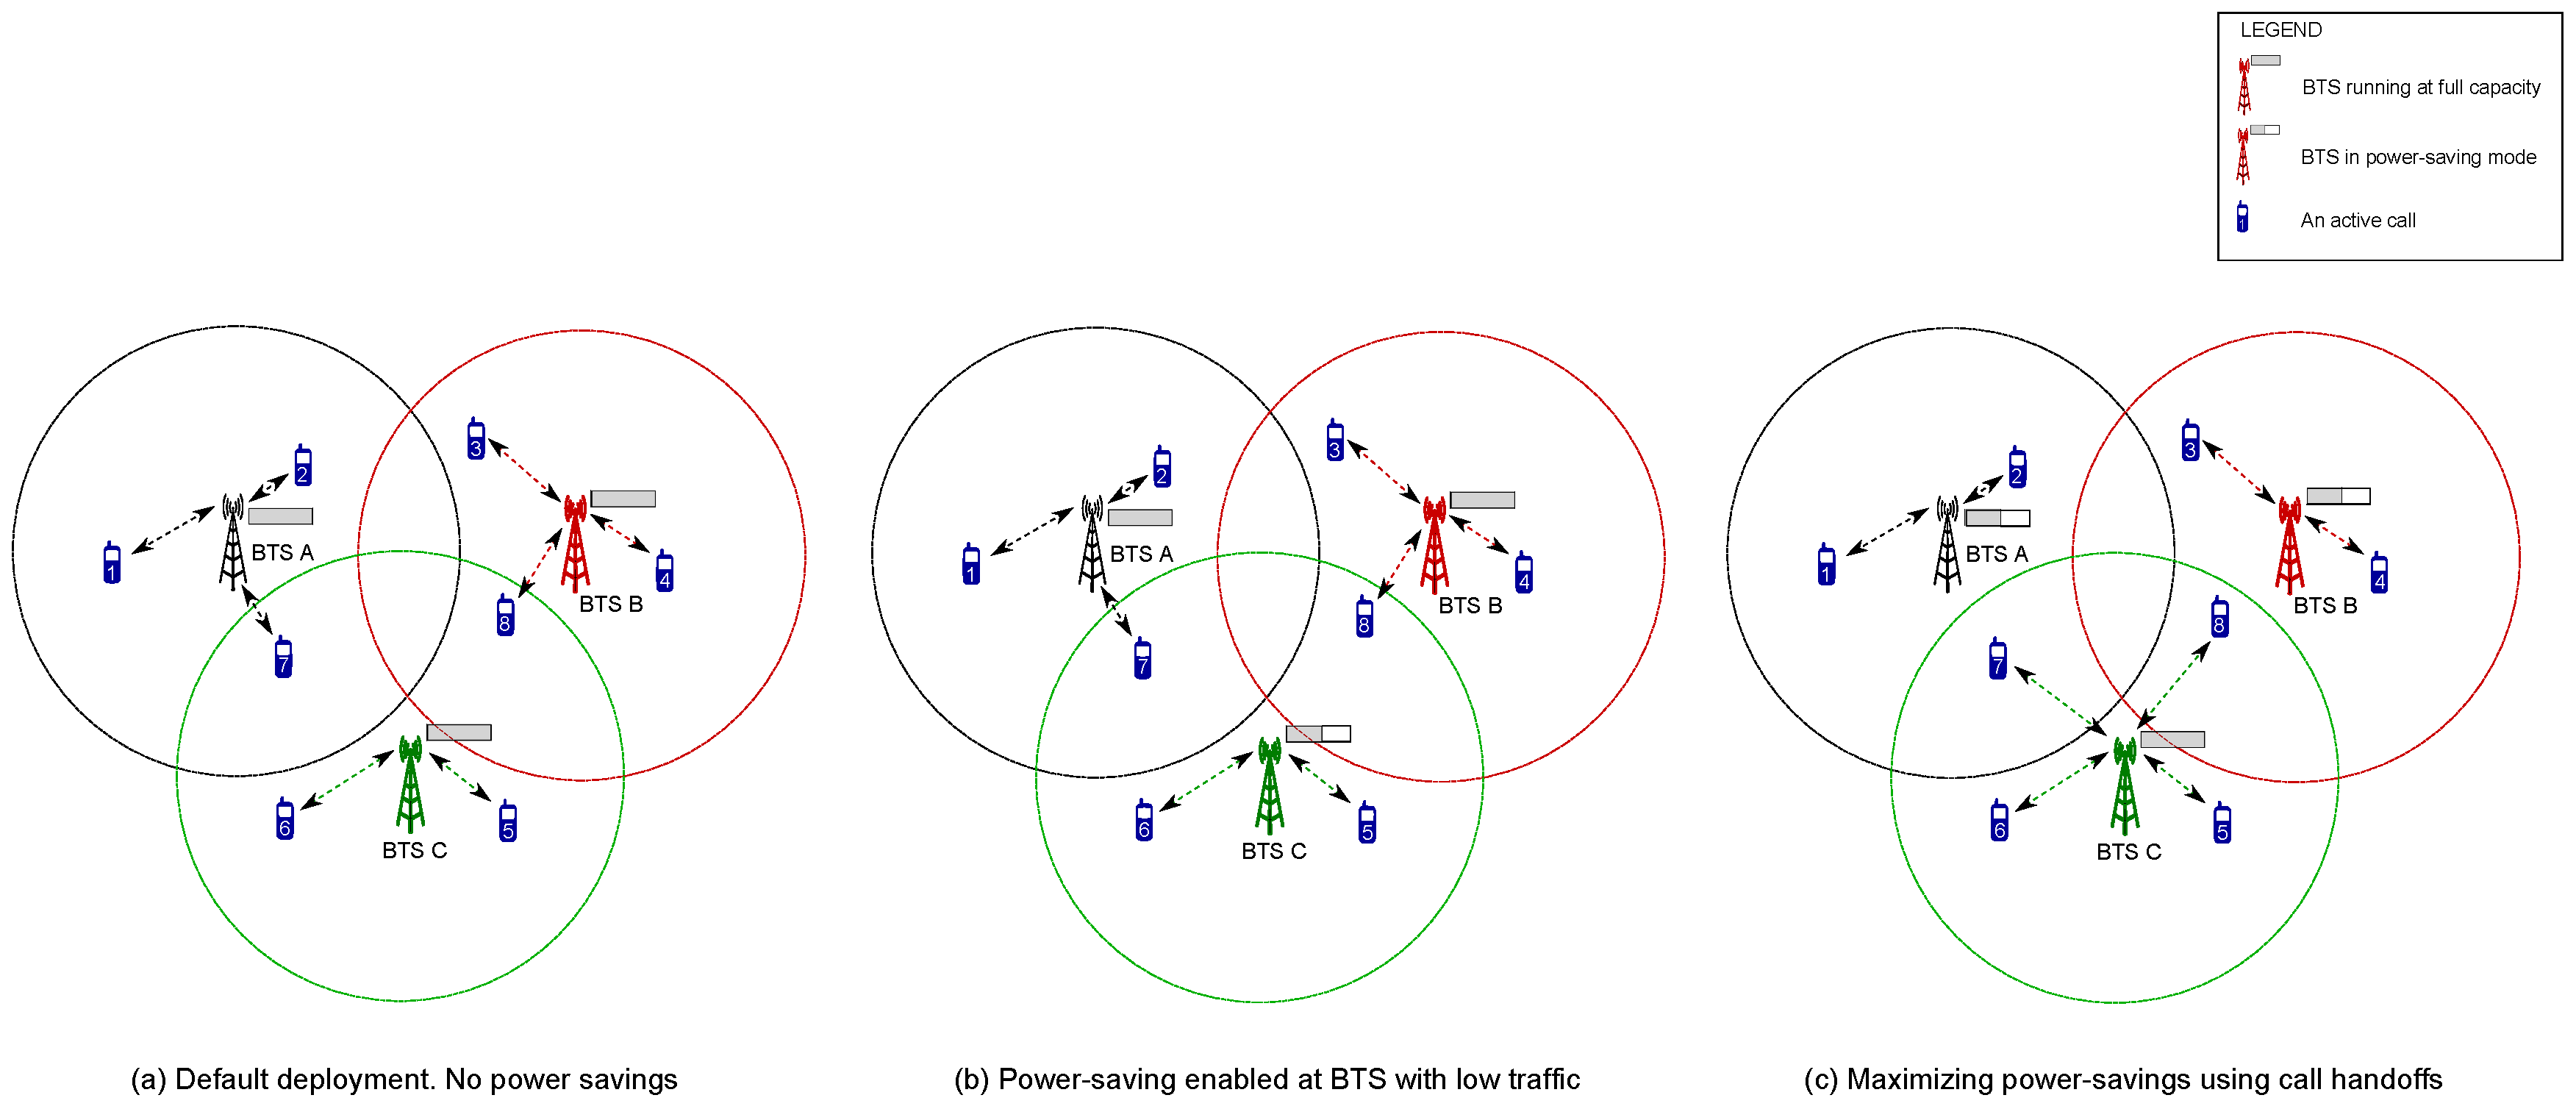
\includegraphics[width=1\textwidth]{figures/illustrationall.eps}
\caption{A toy example to illustrate the main idea behind Low-Carb. Three BTSs (A, B and C) are shown alongwith eight active calls. The serving BTS for each call is shown using a dashed line. A solid completely filled bar alongside a BTS symbol indicates that it is running in the default configuration where all TRXs are enabled. A BTS in power-saving mode is indicated with a half-filled bar next to it. Assume that power-saving mode may be enabled at a BTS if it has less than three active calls. (a) shows the default configuration where power-saving mode is not used. (b) shows the approach currently used by operators whereby power-saving mode is enabled on a BTS with low-traffic. (c) shows our proposed approach, whereby calls may be handed-off to nearby BTSs, thus maximizing the number of BTSs in power-saving mode.}
\label{fig:illustrationall}
\end{figure}


Let us illustrate the main idea behind the energy-saving approach proposed in this paper with the help of the illustration in Figure~\ref{fig:illustrationall}. The figure shows three nearby BTSs collectively serving eight active calls. The association of call to the serving BTS is indicated by means of a dashed line, while the boundary of the potential service area of a BTS is indicated by means of a dashed circle around it. By default, each call is served by the BTS from which the mobile station receives the strongest signal. In this example, we assume that the call handling capacity of each BTS is six simultaneous calls. Furthermore, we assume that the power-saving threshold is three calls, i.e., if a BTS is serving less than three calls, it may be put into power-saving mode. In Figure~\ref{fig:illustrationall}, a BTS in it's default configuration, i.e., all TRXs enabled is indicated with a solid bar next to the BTS symbol. Meanwhile, a BTS in power-saving mode is shown by a half-filled bar next to the BTS symbol.


In Figure~\ref{fig:illustrationall}, note that calls 1 through 6 each have only one candidate serving BTS, while call 7 may be served either by BTS A or C and call 8 may be served either by BTS B or C. Figure~\ref{fig:illustrationall} (a) shows the default deployment with default call routing whereas no power-saving is used. Since BTS C is serving only two calls, it may be placed in power-saving mode. Figure~\ref{fig:illustrationall} (b) shows this network state, which indicates the current practice in operational cellular networks, whereby BTS C is put into power-saving mode because it's current call volume is below the power-saving threshold. However, this is not the optimal call routing strategy in terms of energy-savings. We may handoff calls 7 and 8 to BTS C, thereby reducing the call volume at both BTS A and B below the power-saving threshold. This results in the energy-optimal call routing strategy, proposed in this paper, shown in Figure~\ref{fig:illustrationall} (c). 


This paper presents Low-Carb which combines the \textit{BTS
power saving} with \textit{hand-off}, another commonly used
feature in cellular networks that facilitates user movement
from one location to another. Low-Carb proposes to hand-off
calls from one BTS to another, without making a negative impact
on the network quality of service, such that the \textit{BTS
power savings} can be applied to a maximal number of base
stations throughout the cellular network. As compared to the
use of uncoordinated \textit{BTS power savings}, Low-Carb
offers additional power savings as it may allow a larger number
of TRXs to be deactivated. 
In present day deployments, this is possible since most callers
receive sufficiently strong signal from several nearby
BTSs~\cite{Peng:2011:BTSSaving:Mobicom}. Fig.~\ref{fig:btscdf}
shows coverage diversity evident in the urban data from a large
cellular provider that we used in our evaluations; one can see
that about half of the callers have 3 or more candidates for
serving BTS. Furthermore, neighboring sites can have different traffic loads at a given time. Fig.~\ref{fig:traffic}, for instance, shows normalized traffic at two neighboring sites in our dataset for a 24 hour period. Thus, some calls may be handed off from busy BTSs to nearby BTSs with lower traffic volume to increase the number of BTSs in power-saving mode.

\begin{figure}
\centering
\subfigure[]{
\includegraphics[width=0.48\textwidth]{figures/coveragecdf.eps}
\label{fig:btscdf}
}
\subfigure[]{\includegraphics[width=0.48\textwidth]{figures/traffic.eps}
\label{fig:traffic}
}
\caption{Characteristics of our dataset: (a) Empirical CDF of the number of potential serving BTSs for a call in our dataset (large metropolitan area), (b) Normalized traffic intensity at two neighboring sites in our dataset} 
\label{fig:trafficmodelstats}
\end{figure}

We formulate an optimization problem to minimize the power
consumption in a GSM network by shuffling active calls between
nearby BTSs while keeping in check the MS uplink budget and without dropping any active calls. By constraining the uplink budget, we ensure that call quality is not adversely affected. 

In a shorter version of this paper~\cite{ilyas:lowcarb:globecom13}, we made the following contributions:
\begin{enumerate}
\item We formulated, Low-Carb, a mathematical optimization problem to maximize energy savings in a cellular network such that call quality is not compromised. To maximize energy savings, Low-Carb relies on two features that are implemented in typical BTS hardware and are commonly used by cellular operators, albeit in a non-systematic manner.
\item Since our formulation of Low-Carb is NP-Hard, we provided a heuristic algorithm for solving the Low-Carb problem.
\item We used real data sets from a large GSM network operator in Pakistan to evaluate Low-Carb's utility.
\end{enumerate}
In this paper, we extend our prior work to make the following additional contributions:

\begin{enumerate}
\item Let $\delta$ be the traffic capacity of the BTS in low-power mode. If the BTS is placed in power-saving mode as soon as the traffic reaches $\delta - 1$ calls, then there may be several oscillations in and out of low-power mode due to short-term traffic variations. During these oscillations, some calls may be blocked as well, which is undesirable. Thus, traffic must be allowed to fall to at least $\delta - \epsilon$ calls before the BTS is put into low-power mode. If we pick a high value for $\epsilon$, the amount of energy savings is expected to drop. We experiment with various values for $\epsilon$ and study the dependence of the amount of energy savings on the value of $\epsilon$.
\item In~\cite{ilyas:lowcarb:globecom13}, we had considered that a BTS could be put into one of two possible states, namely low-power and high-power mode. In this paper, we consider that a BTS may operate in one of six modes of operation in terms of its power consumption. We show that a higher granularity of number of BTS operational states results in greater energy savings.
\item We provide another heuristic algorithm for solving Low-Carb which is different from the one presented in the shorter version of this paper.
\end{enumerate}
The rest of the paper is structured as follows. The formulation
of Low-Carb optimization problem is given in
section~\ref{sec:formulation}. Experimental setup and the
results are presented in sections~\ref{sec:expermintalsetup}
and~\ref{sec:results}, respectively. In
section~\ref{sec:conclusions}, we draw the conclusions
highlighting the power saving strategy for service providers.
\section{Related Work}
\label{sec:related} 
The problem that we investigated in this work falls into the broad category of resource scheduling problem under constraints. Resource scheduling problem occurs in many different domains whereby similar solution strategies are applicable. Some examples of prior work in other domains on similar problems include resource provisioning in data centers~\cite{Jeyarani:2012:DIA:2148243.2148374,serverEnergy,Mazzucco:Maximizing:2011:CoRR,Oh:2011:ECS:2170444.2170458,Chase:2001:MES:502059.502045}, scheduling in compute clusters~\cite{AlDaoud2012745}, System on Chip (SOC)~\cite{Fang:2011:COP:1995896.1995940}, electric power systems and smart grid~\cite{Javed:2008:ULP:1485753.1485792,Logenthiran2011138,Celli:2001:PICA,FahadJavedAdOpt.SASO.2009.26}, WiFi access points~\cite{Marsan:2010:SAM:1791314.1791340}, wide area networks~\cite{Cavdar:2011:ECOC}, high performance computing~\cite{Lee:ServerConsolidation:2011:Globecom,Pinheiro01loadbalancing,Yao:DCPowerReduction:2012:INFOCOM,Herodotou:Starfish:2011:CIDR,Herodotou:2011:NOS:2038916.2038934,Aikema:ElecCostHPC:2011:ISSST} as well as cellular networks~\cite{Peng:2011:TPS:2030613.2030628,Peng:2011:BTSSaving:Mobicom}.

Our focus in the present work is to develop techniques that are practically usable in operational networks instead of taking a clean-slate approach. In this sense, it differs from much prior work in energy efficiency in cellular networks. A key benefit of this approach is that it 
does not require any additional hardware
and works within the GSM specifications. Our
work is very similar in spirit to the concept of
\textit{frequency dimming}
in~\cite{Tipper:Dimming:Globecom:2010} albeit at a different
level of abstraction. A similar approach is also proposed
in~\cite{Blume:2010:BLTJ:CellularPower} with some rough
estimates of expected savings. We, on the other hand, use site
locations and traffic traces from a large cellular network with
more than 13 million subscribers to run a simulation study
assessing the benefits of dynamic equipment scaling coupled
with call hand-offs. 
\section{Problem Formulation}
\label{sec:formulation}
\subsection{Single Base Transceiver Station (BTS)}
Power consumed by a BTS, as a function of traffic load, can be
well approximated as a linear curve with a non-zero
y-intercept~\cite{Peng:2011:BTSSaving:Mobicom} given as
$P_1+l(P_2-P_1)/t_{max}$. Here $P_1$ and $P_2$ are the power
consumption at no load and full load, respectively, $l$ is the
number of calls presently being handled, and $t_{max}$ is the
maximum number of calls that can be handled.

Let $\delta$ be the traffic threshold at which the \textit{BTS
power savings} is applied (i.e., when BTS deactivates some TRXs
moving into low-power mode). Since all TRXs are identical, the
per call increase in power consumption, and hence the slope of
the power consumption profile in Fig.~\ref{fig:powermodel1},
remains the same whether or not some TRXs are deactivated. As
also indicated in Fig.~\ref{fig:powermodel1}, the no-load power
consumption drops to $P_1-\gamma$ in the low-power mode, where
$\gamma$ is a constant that depends on the equipment type and
the number of TRXs deactivated.

If $x$ is an indicator variable which is 1 when \textit{BTS
power savings} is applied, and $0$ otherwise, then the BTS
power consumption may be given by $P_1+l(P_2-P_1)/t_{max} -
(1-x)\gamma$, also indicated in Fig.~\ref{fig:powermodel1} by
the piecewise linear solid line.

\begin{figure}
\centering
\includegraphics[width=0.46\textwidth]{figures/powermodel.eps}
\caption{BTS power consumption model. Low-power (BTS power savings) mode is optional and kicks in at low loads.}
\label{fig:powermodel1}
\end{figure}

The granularity of TRX deactivation can be increased to give the power consumption model in Fig.~\ref{fig:powermodel2}. If the traffic is above threshold $\delta_2$, the BTS operates in the default high-power mode. When the traffic drops below threshold $\delta_2$, two TRXs are power-gated, and the BTS enter the medium-power mode (4+4+4 configuration). When the traffic falls below threshold $\delta_1$, two more TRXs are power-gated and the BTS enters the low-power mode.

\begin{figure}
\centering
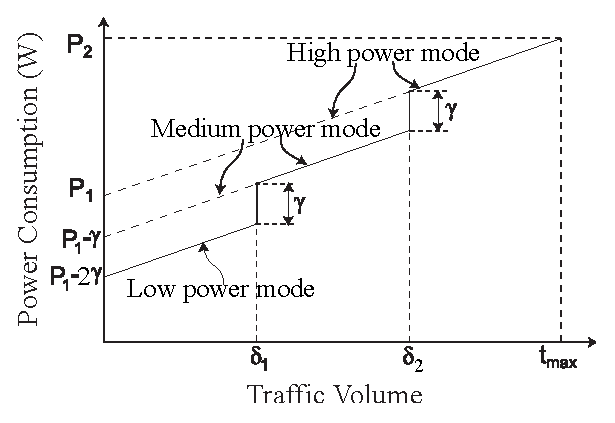
\includegraphics[width=0.46\textwidth]{figures/powermodel2.eps}
\caption{BTS power consumption model. BTS power saving is applied in a more granular way.}
\label{fig:powermodel2}
\end{figure}

The less granular model of Fig.~\ref{fig:powermodel1} offers energy saving potential only when traffic falls to about one-third of the BTS capacity. The more granular model of Fig.~\ref{fig:powermodel2}, on the other hand offers energy savings in two steps, with the first one kicking in as soon as the traffic falls below approximately two-third of the BTS traffic capacity. Therefore, the more granular model (Fig.~\ref{fig:powermodel2}) should be more attractive for energy savings than the less granular one (Fig.~\ref{fig:powerm odel1}).

\subsection{Multi-BTS Cellular Setting}
Consider an area with $n$ active callers being served by $m$ BTSs.
We introduce indicator variable $w_{i,j}$, which is $1$ if call
$i$ \textit{is being} handled at BTS $j$ and $0$ otherwise. We
assume availability of an $n\times m$ matrix whose entry
$c_{i,j}$ is $1$ if caller $i$ \textit{can be} served through
BTS $j$ without exceeding the uplink or downlink budgets.
This information can be extracted by the data periodically
transmitted by each MS comprising the received signal strength
from nearby BTSs during a call. We also introduce indicator
variable $x_j$, which is $1$ if BTS $j$ is operating in
high-power mode (i.e., without \textit{BTS power savings}) and
$0$ otherwise. Using these variables and parameters, we can
formulate an optimization problem to minimize the total power
consumption over the network as:
\begin{align}
\textit{minimize} \quad \sum_{j=1}^{m} \left[
P_1+\sum_{i=1}^{n}\frac{w_{i,j}(P_2-P_1)}{t_{max}}-(1-x_j)\gamma
\right]
\end{align}
subject to the following constraints:
\begin{align}
& \sum_{j=1}^m w_{i,j} = 1 \qquad \forall i \\
& w_{i,j} \leq c_{i,j} \qquad \forall i, j \\
& \sum_{i=1}^nw_{i,j}-\delta \leq Mx_j \qquad \forall j%\\
\end{align}
\begin{align}
& \sum_{i=1}^n w_{i,j} \le t_{max} \qquad \forall i \\
%\end{align}
%\begin{align}
& w_{i,j}, x_j \in {0,1} \qquad \forall i, j%\\
%x_j \in {0,1}
\end{align}

We call this optimization problem, the two-step Low-Carb problem. The objective function is a simple generalization from the case
of one BTS. The first constraint ensures that no active call is
dropped just to save on power. The second constraint secures
the uplink budget by ensuring that no call is routed to a BTS
that can not handle it. The third constraint picks the correct
value for the decision variable $x_j$. The fourth constraint is the capacity constraint on all BTSs, while the last
constraint is the binary value constraint on the decision
variables.

For the three-step BTS power-saving model of Fig.~\ref{fig:powermodel2}, the optimization problem can be stated as:
\begin{align}
\textit{minimize} \quad \sum_{j=1}^{m} \left[
P_1+\sum_{i=1}^{n}\frac{w_{i,j}(P_2-P_1)}{t_{max}}-\frac{(1-x_j)\gamma}{2}-\frac{(1-y_j)\gamma}{2}
\right]
\end{align}
subject to the following constraints:
\begin{align}
& \sum_{j=1}^m w_{i,j} = 1 \qquad \forall i \\
& w_{i,j} \leq c_{i,j} \qquad \forall i, j \\
& \sum_{i=1}^nw_{i,j}-\delta_1 \leq Mx_j \qquad \forall j\\
& \sum_{i=1}^nw_{i,j}-\delta_2 \leq My_j \qquad \forall j\\
%\end{align}
%\begin{align}
& \sum_{i=1}^n w_{i,j} \le t_{max} \qquad \forall i \\
%\end{align}
%\begin{align}
& w_{i,j}, x_j, y_j\in {0,1} \qquad \forall i, j%\\
%x_j \in {0,1}
\end{align}

In the above statement, we've added an indicator variable $y_j$, which is $1$ if BTS $j$ is in medium-power mode, $0$ otherwise. The fourth constraints ensures that $y_j$ takes on the proper value depending on the current traffic volume at BTS $j$. We call this optimization problem the three-step Low-Carb problem.


\subsection{Heuristic solutions to Low-Carb}
\label{subsec:heuristics} Both of the above optimization problems are Binary Integer Programs
(BIP), which is NP-Hard. It is intractable to solve it for an
operator's entire network, but solving it for a subset of the
network will provide some estimates of the amount of energy
savings possible using Low-Carb. Deployment to large operator
networks would require approximation algorithms. In this paper, we present two heuristics to solve the problem approximately and compare the results with the optimal solution.

\subsubsection{Heuristic 1}
\label{subsubsec:heuristic1} We describe here, the first heuristic for the two-step Low-Carb problem. Our first heuristic divides the set of BTSs $B$, into two disjoint subsets $B_1$ and $B_2$. Subset $B_1$ consists of those BTSs that have traffic above threshold $delta$. Subset $B_2$ consists of all other BTSs. Our heuristic shuffles the members of $B_1$ and iterates over the set. In every iteration, our heuristic looks at the current traffic load at a particular BTS. Let this traffic load be $h$. The heuristic declares that it must hand-off $h$-$delta$ calls away from the current BTS to it's neighbors in the subset $B_2$ while ensuring that no BTS in $B_2$ leaves it's subset as a result of the hand-off. This heuristic can be invoked multiple times, using a different shuffled order of BTSs in $B_2$ to improve the heuristic's performance. At the end of this process, members of $B_2$ are placed in low-power mode. 


For the three-step Low-Carb problem, members of $B_1$ are those BTSs that have traffic above threshold $delta_2$, while $B_2$ contains all other BTSs. We shuffle some calls from BTSs selected in a random order attempting to reduce the cardinality of set $B_1$. Once we are done iterating over all members of $B_1$, we re-initialize $B_1$ to contain BTSs that have traffic above threshold $delta_1$ and $B_2$ to contain all other BTSs and repeat the same call hand-off process as described earlier. In the end, those BTSs that have traffic above $\delta_1$ but below $\delta_2$ are placed in the medium-power mode while those with traffic below the $\delta_1$ threshold are palced in the low-power mode. Once again, this heuristic can be invoked multiple times to improve the probability of finding a near-optimal solution.

\subsubsection{Heuristic 2}
\label{subsubsec:heuristic2} We first describe the second heuristic for the two-step Low-Carb problem. In contrast to the first heuristic, the second one iterates over calls first. It first assigns all calls that only have one candidate BTS to the only BTS that can handle them.
\section{Experimental Setup}
\label{sec:expermintalsetup}

\section{Results}
\label{sec:results}
The following results were obtained through simulation experiments driven by real traffic traces and deployment geography. The experiments perform a combination of activation of BTS power-saving mode on BTSs alongwith a periodic update of serving BTS for each active call, such that the instantaneous energy consumption in the network is minimized.

First, we consider the benefit of BTS power-saving alone, resulting from traffic diversity at each BTS compared to running the network in the default configuration. The percentage reduction in energy consumption is listed in table~\ref{tab:psonly}. The results indicate that a saving of between 4\% and 12\% can be achieved in a network just by activating BTS power savings. We note here that some of these results are in agreement with Ericsson's claim of saving 10-20\% energy by using BTS power-saving on Germany's Vodafone network~\cite{ericssonclaim}. 

In absolute terms, this represents a cumulative saving of between 43 kWh and 217 kWh per day on 26 BTSs. Now, consider that there are five cellular oeprators in Pakistan: Mobilink with more than 8500 sites~\cite{mobilinksitecount}, Ufone with more than 8000 sites~\cite{ptaannreport}, Zong with more than 5500 sites~\cite{ptaannreport}, Telenor with more than 7000 sites~\cite{telenorsitecount} and Warid with more than 4500 sites~\cite{ptaannreport}. Overall, there were more than 31000 sites in Pakistan at the end of 2011. We extrapolated the daily energy savings number over 26 BTSs to calculate the daily energy savings possible for a country like Pakistan with over 31000 BTSs (see the last row of table~\ref{tab:psonly}). The results indicate that mere activation of BTS power saving option itself can save quite a bit of electrical energy, a critical resource, especially in a developing country. As we shall see next, greater energy savings are possible if we couple periodical call shuffling with BTS power savings in the network. 

\begin{table}
\centering
\begin{tabular}{|c|c|c|c|}
\hline Energy saving & Model 1 & Model 2 & Model 3 \\
\hline Percentage & 4.73\% & 5.43\% & 12.89\% \\
\hline Daily absolute saving & 43.28 & 109.68 & 217.12 \\
over 26 BTSs (in kWh) & \ & \ & \ \\
\hline Country-wide daily saving & 51.6 & 130.77 & 258.87\\
over 31000 sites (in MWh) & \ & \ & \ \\
\hline
\end{tabular}
\caption{Energy savings by using BTS power savings only}
\label{tab:psonly}
\end{table}


If periodic optimization of call placement is coupled with BTS power-saving, the energy saving improves, as shown in Fig.~\ref{fig:results2}.
%As noted earlier, we expect to achieve greater energy savings by periodically handing-off calls from busier BTSs to nearby BTSs with lower traffic to put a maximal number of BTSs in power-saving mode. If the periodic re-optimization is done aggressively, the network would remain in a nearly optimal state more often. On the other hand, a less aggressive policy would have the network in a nearly optimal state less often. We, therefore, expect that savings in power consumption should increase when the interval between re-optimization episodes is decreased. Since we are interested in the overall impact of the power saving scheme, the percentage power savings are computed over the entire network and not per BTS. %Furthermore, the percentage savings are computed over the default mapping of calls to BTSs, i.e., each call is associated with the BTS that the caller receives the strongest radio signal from.
%
%The percentage reduction achieved by using Low-Carb for the three BTS models is plotted in Fig.~\ref{fig:results2}. 
For all three BTS models, we see an almost linear increase in power saving as the duration of the re-optimization interval is decreased. Recall that the three models are significantly different in terms of power consumption (see Table~\ref{tab:models}). We can not directly say that because model 3 BTS offers the highest percentage reduction in energy consumption, it also saves the most energy (in kWh). %The results in Fig.~\ref{fig:results2} are quite useful to study the sensitivity of Low-Carb to the duration of re-optimization interval. However, one can't compare the three BTS models based on that, because the power consumption profiles are different for the three. For instance, a $15\%$ saving on $100kWh$ is not the same as a $15\%$ power saving on $500kWh$.

%\begin{figure}
%\includegraphics[width=0.5\textwidth]{figures/percent.savings.powersaving.eps}
%\caption{Percentage reduction in power consumption vs re-optimization interval - BTS Power Saving only}
%\label{fig:results1}
%\end{figure}

\begin{figure}
\includegraphics[width=0.45\textwidth]{figures/percent.savings.powersaving.eps}
\caption{Percent reduction in energy consumption vs re-optimization interval}
\label{fig:results2}
\end{figure}

%\begin{figure}
%\includegraphics[width=0.5\textwidth]{figures/e.savings.powersaving.eps}
%\caption{Reduction in energy consumption through BTS Power Saving}
%\label{fig:results3}
%\end{figure}

To \textit{compare} the three BTS models in terms of energy saving potential, we also present the absolute reduction in energy consumption for the three BTS models in Fig.~\ref{fig:results4}. We see the same linear trend alongwith the same relative order of the three models in terms of amount of saved energy, as in Fig.~\ref{fig:results2}. 

Re-optimizing at an interval less than the mean call duration should offer greater savings than a less frequent re-optimization, because the former regime has the opportunity to optimize more by handing off most of the calls. This is confirmed in our results. For instance, for model 1 BTS, the gain in energy savings going from a 60 minutes inter-optimization interval to 30 minutes gains an energy saving of only 0.0506 kWh per minute, while decreasing the inter-optimization interval from 2 minutes to 1 minute gains 12.5421 kWh. %We notice a more pronounced separation between the three models in Fig.~\ref{fig:results4}, resulting from the considerable difference between the maximum and minimum power consumption levels for the three models, as well as the values of $\gamma$.

\begin{figure}
\includegraphics[width=0.45\textwidth]{figures/e.savings.powersaving.eps}
\caption{Reduction in energy consumption vs re-optimization interval}
\label{fig:results4}
\end{figure}

Let us now interpret what these results mean physically in terms of ecological impact. If we extrapolate our results, the total energy saving for Pakistan are projected to be $60.72$ MWh, $156.84$ MWh and $301.61$ MWh daily, respectively, according to the three BTS models. These savings in energy are significant, especially for small and developing countries. Since network deployments and traffic patterns are similar in different countries, we also expect that similar savings should be achievable in many other countries as well.

In the above extrapolation, we have assumed that the same amount of energy saving would be applicable in rural as well as urban settings. While this may not necessarily be true because the deployments are sparse in rural settings, resulting in reduced potential to save energy by means of call hand-off to neighboring sites, the potential to save energy merely by BTS power-saving should be higher in a rural setting because traffic loads are typically lower.
%An assumption in the above extrapolation is that the same amount of energy can be saved anywhere in the network. However, traffic patterns and deployment denisty vary in a given network. For instance, cellular networks in rural areas are typically characterized by lower traffic alongwith sparse deployments and, therefore, may not offer as much energy saving possibility as an urban setting (our dataset is for an urban setting). We do not expect that there would be no opportunity for energy savings in rural settings, because of multiple factors. This is partially correct because saving more energy by call-handoff is tough due to sparse deployments. However, the traffic is typically low in such areas, so there should be a greater opportunity to deactivate TRXs most of the time, resulting in greater savings in rural areas than urban. In an extended version of this paper, we will experiment with a dataset from a live network in a rural setting to assess the overall savings possible in a country-wide network.

%\begin{figure}
%\includegraphics[width=0.5\textwidth]{figures/improvementplot.eps}
%\caption{Percentage reduction in power consumption vs re-optimization interval - Sparse deployment of $9$ BTSs}
%\label{fig:results1}
%\end{figure}
%
%For a region with sparse deployments, we plot the percentage savings in power consumption as the re-optimization interval was varied, in Fig.~\ref{fig:results1}. For model 1 BTS, we were only able to reduce the power consumption by about $2.5\%$ even if we re-optimized once every minute. This is expected because placing a BTS in power saving mode affords a saving of $240W$ (the value of $\gamma$), which is a small percentage of the maximum power consumption($1500W$) and this small saving is applicable only while the traffic at a BTS is below $\delta$.
%
%The percentage savings for model 2 BTS are somewhat better than those for the model 1 BTS. This would be due to the value of  $\gamma$ being a larger fraction of the overall site power consumption than model 1. For model 3 BTS, the value of $\gamma$ is a pretty large fraction of the overall site configuration, so as expected, we see larger overall percentage reduction in power consumption.
%
%A comparison of energy savings for the three BTS types using percentage energy savings does not give the whole picture because the overall power consumption of the three types are different. To put the savings in perspective, we plot the amount of energy (kWh) saved per day over $9$ BTSs, using the proposed scheme. For the sparse deployment, the results are plotted in Fig.~\ref{fig:results2}.
% 
%\begin{figure}
%\includegraphics[width=0.5\textwidth]{figures/energysavingssparse.eps}
%\caption{Amount of energy saved per day (kWh) - Sparse deployment of $9$ BTSs}
%\label{fig:results2}
%\end{figure}
%
%We can see the same pattern in the amount of energy saved for the three models as we did for the percentage reduction in power consumption, albeit with model 2 differentiating itself somewhat more clearly from model 1. This is clearly because there is a large difference between the maximum power consumption for model 1 and 2.
%
%One can see in Fig.~\ref{fig:results2} that when re-optimization is done every $5$ minutes, one may be able to save approximately $2.5kWh$, $7kWh$ and $15kWh$ respectively with model 1, 2 and 3. This saving is achieved over a set of $9$ BTSs. In order to understand what kind of savings this translates into for an operator in a country like Pakistan, consider that for an operator named Telenor that has over $7000$ sites in Pakistan~\cite{telenorsitecount} $1800MHz$ band, our results approximate a daily saving of $105MWh$.
%
%For a dense deployment of $9$ BTSs, results of the same set of experiments are plotted in Fig.~\ref{fig:results3} and Fig.~\ref{fig:results4}. These graphs show the same trends as observed for the sparse deployment but with greater magnitudes. For a dense deployment, for instance, when optimizing every $5$ minutes, the savings afforded in a dense deployment for model 3 were about $10kWh$ per day.
%
%\begin{figure}
%\includegraphics[width=0.5\textwidth]{figures/improvementplotdense.eps}
%\caption{Percentage reduction in power consumption vs re-optimization interval - Dense deployment of $9$ BTSs}
%\label{fig:results3}
%\end{figure}
%
%\begin{figure}
%\includegraphics[width=0.5\textwidth]{figures/energysavingsdense.eps}
%\caption{Amount of energy saved per day (kWh) - Dense deployment of $9$ BTSs}
%\label{fig:results4}
%\end{figure}
%
%An operator's network is typically a mix of sparse and dense deployments depending on the spread of subscriber density in their coverage area. For a range of sparse/dense deployment mixes, we computed the approximate achievable reduction in annual energy consumption using the proposed technique. This calculation is just a weighted average of the energy consumption reduction for the sparse and dense deployment as obtained in our experiments. To conserve space, we are listing results only for the case when re-optimization is done every $5$ minutes. The results are listed in table~\ref{tab:benefits}.
%
%\begin{table*}
%\centering
%\begin{tabular}{|c|c|c|c|c|c|c|c|c|c|}
%\hline BTS Model & \multicolumn{9}{|c|}{Sparse/Dense deployment mix (percentages)}\\
%\cline{2-10} \ & 10/90 & 20/80 & 30/70 & 40/60 & 50/50 & 60/40 & 70/30 & 80/20 & 90/10\\
%\hline 1 & 27.58 &	26.77 &	25.97 & 25.16 & 24.35 &	23.55 &	22.74 &	21.94 &	21.13 \\
%\hline 2 & 69.81	& 67.88	& 65.96	& 64.04	& 62.12	& 60.19	& 58.28 & 56.35	& 54.43 \\
%\hline 3 & 144.39 & 139.66	& 134.93	& 130.19	& 125.45	& 120.72	& 115.98	& 111.24	& 106.51
% \\
%\hline
%\end{tabular}
%\caption{Estimated annual energy savings (MWh) for $7000$ sites in \\ various mixes of sparse and dense deployment}
%\label{tab:benefits}
%\end{table*}

%It is important to consider the cost of this scheme if it is to be deployed in practice. On average, each re-optimization took an average of about one minute when run on a laptop computer with a Core i3 processor and 4 GB of RAM, for the 26 BTS dataset that we considered. Further improvements in running time alongwith joint optimization of a greater number of sites simultaneously can be achieved through a more powerful computer and/or parallelization. However, BIP is an NP-Hard problem, so expecting to solve an online optimization of traffic over a city's entire network would be unrealistic. We must, therefore, come up with heuristics to solve this problem sub-optimally. One heuristic, as proposed in this paper is to separately optimize traffic over small sets of BTSs. Other approaches such as approximations to similar classes of problems (such as the assignment problem) and evolutionary algorithms need to be tried and will be explored in an extended version of this paper.
\section{Conclusions}
\label{sec:conclusions}
BTSs account for most of a cellular network's energy consumption. Motivated by the non load-proportionality of BTS energy consumption, prior work proposed shutting down some BTSs when traffic is low. However, network operators are reluctant to do so for a variety of reasons.

To reduce energy consumption, we propose using a commonly available and used feature called BTS power savings that deactivates some TRXs at BTSs that have low traffic. Furthermore, calls may be handed-off from BTSs with higher load to neighboring ones with lighter load to increase the benefits of BTS power-saving.

Using real network topology and traffic traces in a simulation study , we found that merely using BTS power saving in an urban setting can result in considerable energy savings. Moreover, our results also indicate that periodic call-shuffling between BTSs can further reduce energy consumption in existing large GSM networks.
%% The Appendices part is started with the command \appendix;
%% appendix sections are then done as normal sections
%% \appendix

%% \section{}
%% \label{}

%% References
%%
%% Following citation commands can be used in the body text:
%% Usage of \cite is as follows:
%%   \cite{key}         ==>>  [#]
%%   \cite[chap. 2]{key} ==>> [#, chap. 2]
%%

%% References with bibTeX database:

\bibliographystyle{elsarticle-num}
\bibliography{ref}

%% Authors are advised to submit their bibtex database files. They are
%% requested to list a bibtex style file in the manuscript if they do
%% not want to use elsarticle-num.bst.

%% References without bibTeX database:

% \begin{thebibliography}{00}

%% \bibitem must have the following form:
%%   \bibitem{key}...
%%

% \bibitem{}

% \end{thebibliography}


\end{document}
